\label{visor uavViewer}

Una estación en tierra o GCS (\textit{Ground Control Station}) es una estación base donde se recibe la
información generada por un dron y con la que se puede monitorizar y controlar toda la actividad
de este vehículo. Estas estaciones pueden ser fijas o móviles y permiten al operario que maneje el dron
conocer su estado de una manera simple.

En el entorno de JdeRobot existía previamente una estación en tierra para drones desarrollada en C++ llamada UAV-Viewer. Debido a la necesidad de crear un nuevo interfaz que se asemejara más a un mando de un dron real, se decidió implementar una nueva versión. Además ha servido de validación experimental del driver MavLinkServer puesto que se comunica directamente con él para enviarle comandos de movimiento así como recibir posición del GPS.

\section{Diseño}

El desarrollo de la nueva aplicación UAV-Viewer.py se ha realizado en Python 2.7 en vez de C++ por sencillez para que el entorno JdeRobot tuviera más variedad en sus aplicaciones, en vez de hacer un cambio en la interfaz gráfica de la versión de C++. Las principales diferencias entre ambos visores son el lenguaje y el interfaz gráfico. 

El diagrama de entradas y salidas del nodo UAV-Viewer.py se muestra en la Figura \ref{fig:esquemaUav}, en este caso
conectado a dos drivers: MAVLink para conectarse con el drone y CameraServer para conectarse con
la cámara a bordo.

\begin{figure}[H]
  \centering
  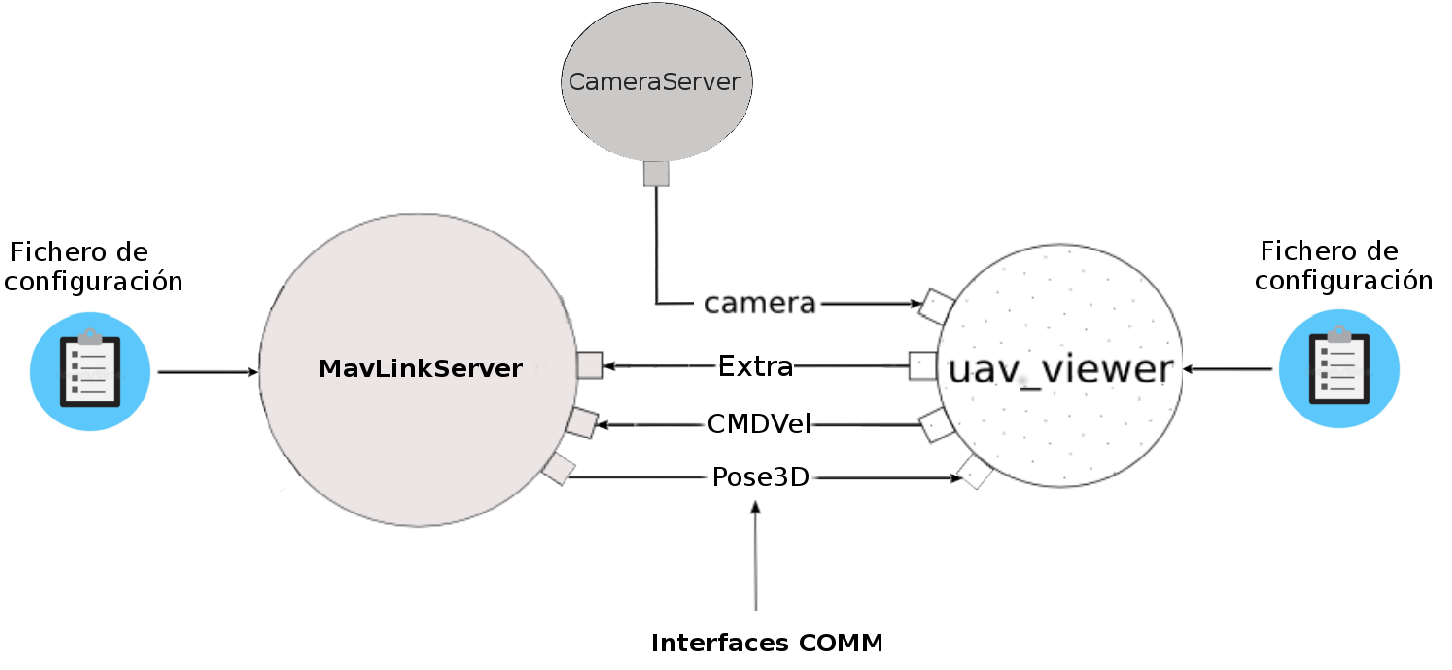
\includegraphics[scale=0.4]{imagenes/MapaGeneral.png}
  \caption{Diagrama de entradas y salidas de UAV-Viewer.py}
  \label{fig:esquemaUav}
\end{figure}

A continuación se muestra el código de inicialización de la aplicación en el cual se inicia la conexión con la biblioteca de mensajes COMM.

\begin{lstlisting}[frame=single]
		#Lectura de la configuracion
        cfg = config.load(sys.argv[1])11

        #Inicializacion de las comunicaciones
        jdrc= comm.init(cfg, 'UAVViewer')

        camera = jdrc.getCameraClient("UAVViewer.Camera")
        navdata = jdrc.getNavdataClient("UAVViewer.Navdata")
        pose = jdrc.getPose3dClient("UAVViewer.Pose3D")
        cmdvel = jdrc.getCMDVelClient("UAVViewer.CMDVel")
        extra = jdrc.getArDroneExtraClient("UAVViewer.Extra")

		#Inicializacion del interfaz grafico y su hebra
        app = QApplication(sys.argv)
        frame = MainWindow()
        frame.setCamera(camera)
        frame.setNavData(navdata)
        frame.setPose3D(pose)
        frame.setCMDVel(cmdvel)
        frame.setExtra(extra)
        frame.show()



        t2 = ThreadGUI(frame)
        t2.daemon=True
        t2.start()
\end{lstlisting}

Existen dos hebras dentro de la aplicación: una controlada por la interfaz de usuario que se encarga de enviar la información de los joysticks y los botones, la otra hebra recibe dicha información, se adecúa dependiendo el estado en el que se encuentre y envía la acción requerida.

La adquisición de imágenes la realiza la hebra encargada de la comunicación con el dron dentro de un bucle de control independiente a la hebra encargada de la interfaz gráfica.  De este modo la hebra encargada de la interfaz gráfica consultará a la hebra que controla el dron periódicamente en busca de nuevas imágenes. Cuando las obtenga, refrescará la imagen que muestra en un determinado periodo de tiempo que puede ser configurado.

\begin{figure}[H]
  \centering
  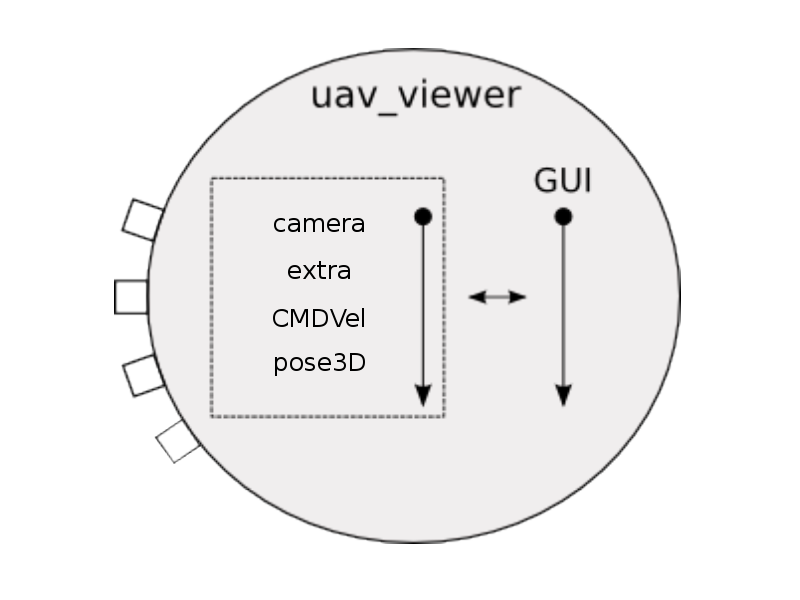
\includegraphics[scale=0.3]{imagenes/uavViewer.png}
  \caption{Hilos Uav-Viewer.py}
  \label{fig:uavViewer}
\end{figure}

\section{Comunicación con drivers} 

Para teleoperar el dron la interfaz gráfica captura los eventos. Estos eventos son creados por los joysticks que envía una señal constante con la velocidad indicada para cada unos de los ejes. La interfaz proporcionada por además de ofrecer el envío de comandos al dron para su control, es capaz de proporcionar los datos de los sensores. A estos datos se los conoce como navdata o datos de navegación. El hilo que comunica Uav viewer con el dron hace uso de ésta interfaz para recibir dichos datos. 

La herramienta se ha diseñado combinando tres bloques como se indica en la figura \ref{fig:memoriaUav}: el de configuración; el de diálogo con el drone, usando interfaces ICE; y el de diálogo con el interfaz de usuario.

\begin{figure}[H]
  \centering
  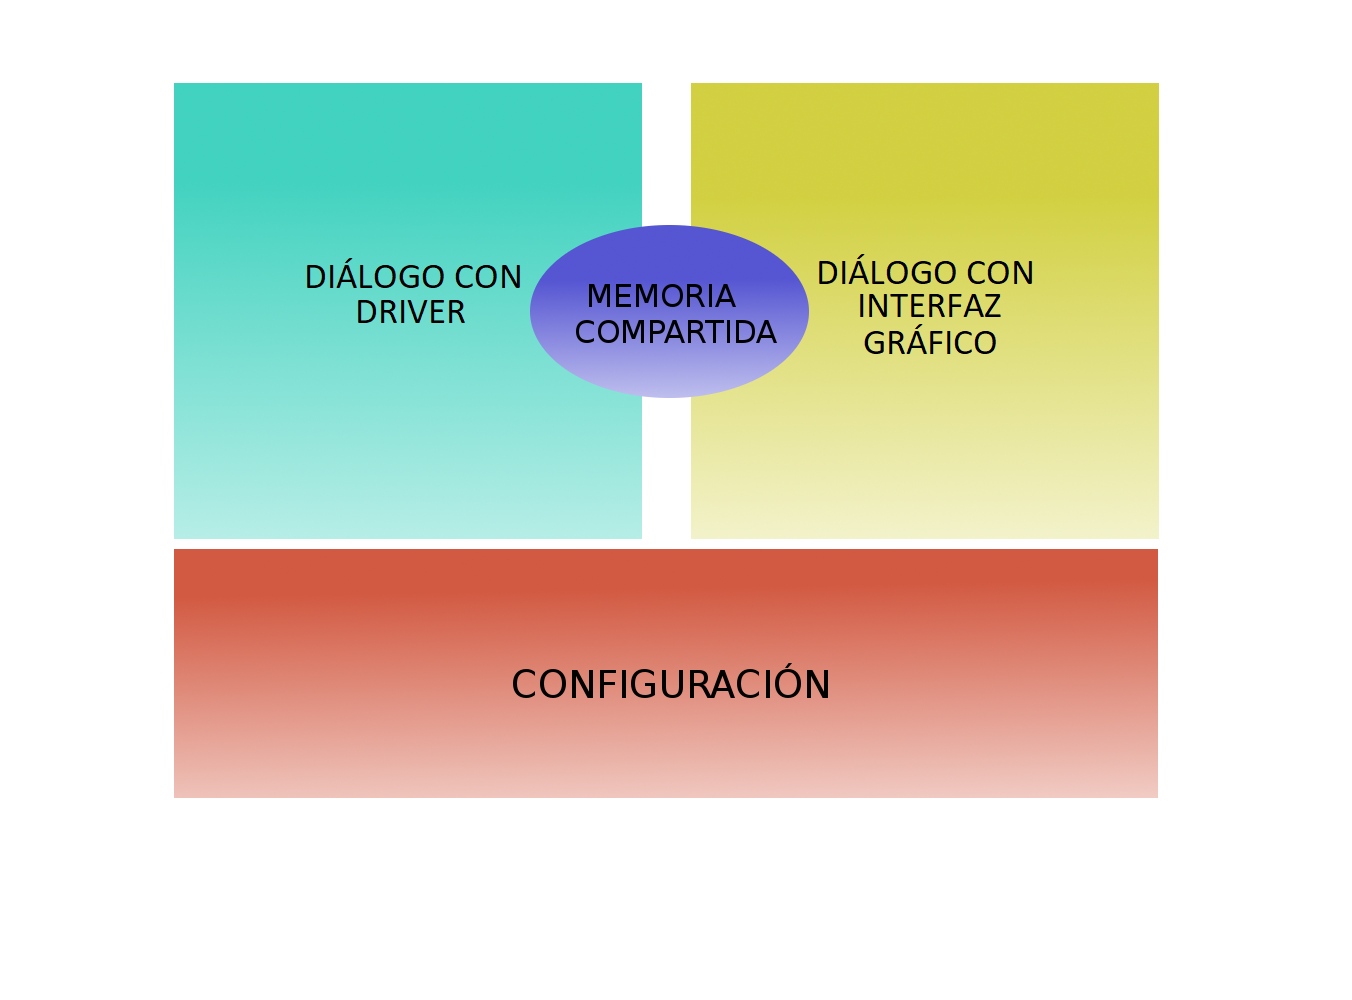
\includegraphics[scale=0.3]{imagenes/MemoriaCompartidaUAV.png}
  \caption{Diagrama de bloques de UAV-Viewer.py}
  \label{fig:memoriaUav}
\end{figure}

Las acciones que envía la interfaz gráfica estan marcadas por ciclos de reloj fijos, cada ciclo actualiza la información necesaria en el interfaz correspondiente. Ha sido necesario el uso de "bloqueos" (\texttt{locks}) para proteger los datos almacenados en la clase y garantizar un acceso en excusión mutua, de igual manera que se utiliza en MAVLinkServer.

\section{Interfaz Gráfica}

La aplicación ha sido desarrollada en python utilizando para el apartado gráfico la librería
para interfaces de usuario Qt. Se ha dividido en tres ventanas: la figura \ref{fig:interfazUavViewer} corresponde a la ventana principal, donde se teleopera el dron. La segunda ventana representa la imagen en tiempo real de la cámara a bordo del dron. Por último, la tercera ventana muestra la información recogida por los sensores del dron, mostrado en la figura \ref{fig:sensores}. A continuación, se describirán las funciones que realiza cada ventana:

La ventana principal se ha realizado de tal manera que se asemeje lo más posible a los mandos de los drones físicos. Las crucetas simulan los joystick de control del dron, de tal forma que el joystick izquierdo controla la altura y el giro (o Yaw), y el joystick derecho controla los ejes X e Y. 

\begin{figure}[H]
  \centering
  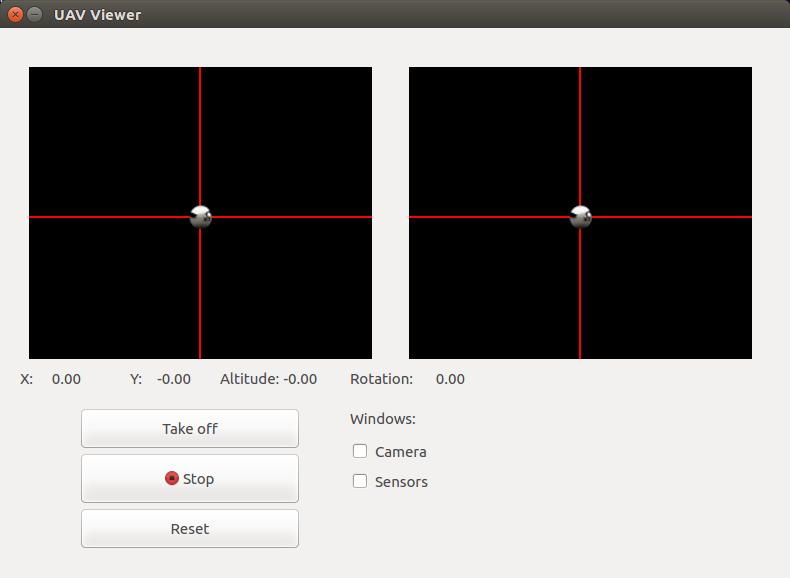
\includegraphics[scale=0.35]{imagenes/Uav_viewer_py.png}
  \caption{Interfaz gráfico de uav-viewer.py para teleoperación}
  \label{fig:interfazUavViewer}
\end{figure}

A su vez, esta ventana dispone de tres botones:
\begin{itemize}
\item \texttt{Take off-Land}: Este botón permite despegar o aterrizar el dron en función del estado de vuelo en el que se encuentre.
\item \texttt{Stop}: Cuadra los joysticks en la posición (0,0) para detener el dron por completo.
\item \texttt{Reset}: Reinicia los valores por defecto: si hubiera alguna ventana auxiliar abierta, cámara o sensores, se cerrarían; además, realiza la misma acción del botón \texttt{Stop}; por último, respetaría el estado de vuelo del dron (la orden \texttt{Take off-Land} no se vería alterada por la acción de este botón).
\end{itemize}

\begin{lstlisting}[frame=single]
 def __init__(self, parent=None):
        super(MainWindow, self).__init__(parent)
        self.setupUi(self)
        self.teleop=TeleopWidget(self,0)
        self.teleop1=TeleopWidget(self,1)
        self.tlLayout.addWidget(self.teleop)
        self.tlLayout_1.addWidget(self.teleop1)
        self.teleop.setVisible(True)

        self.record = False

        self.updGUI.connect(self.updateGUI)

        self.cameraCheck.stateChanged.connect(self.showCameraWidget)
        self.sensorsCheck.stateChanged.connect(self.showSensorsWidget)

        self.cameraWidget = CameraWidget(self)
        self.sensorsWidget = SensorsWidget(self)

        self.cameraCommunicator = Communicator()
        self.trackingCommunicator = Communicator()

        self.stopButton.clicked.connect(self.stopClicked)
        self.resetButton.clicked.connect(self.resetClicked)
        self.takeoffButton.clicked.connect(self.takeOffClicked)
        self.takeoff = False
        self.reset = False
\end{lstlisting}

Además de esta ventana principal, la aplicación desarrollada también implementa la visualización de cámara y de los sensores a bordo. Obtiene las imágenes a través de la interfaz camera. Con la imagen y los metadatos de ésta recuperados desde el driver que suministra las imágenes, UAV-viewer.py la transforma en una imagen compatible con Qt. En función de la cámara activa el tamaño de la ventana donde se muestran las imágenes cambiará para ajustarse al ancho y alto de la imagen obtenida.

\begin{figure}[H]
  \centering
  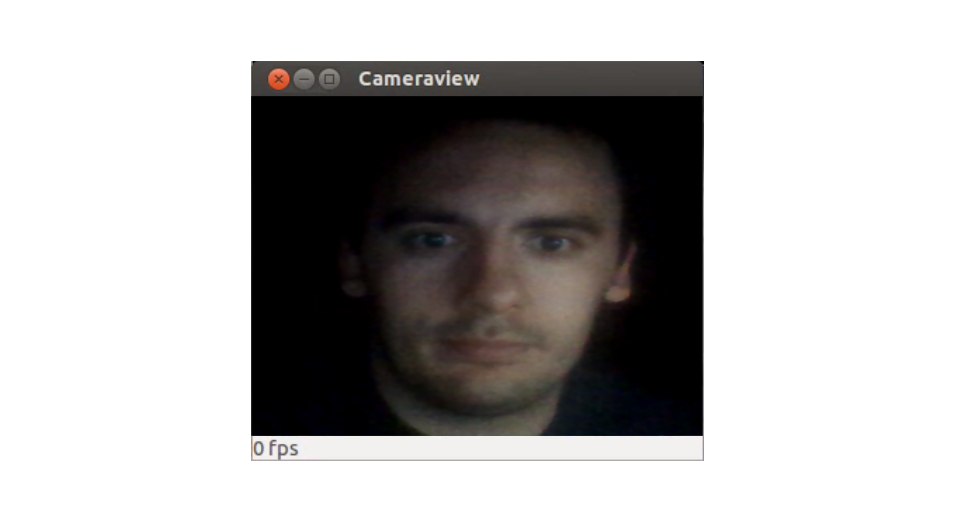
\includegraphics[scale=0.4]{imagenes/cameraView.png}
  \caption{Interfaz gráfico de uav-viewer.py para mostrar la cámara}
  \label{fig:cameraView}
\end{figure}

En la figura \ref{fig:sensores} se puede apreciar cómo el hilo que gestiona la interfaz de usuario rellena varios objetos gráficos con los datos sensoriales obtenidos a través del driver del dron. Podemos ver el porcentaje de batería restante, la altitud del dron, con el indicador de actitud se visualiza fácilmente el alabeo y el cabeceo. Además cuenta con tres velocímetros para indicar la velocidad medida en cada eje. Si esta velocidad es positiva la etiqueta de la velocidad será verde, mientras que si la velocidad es negativa, la etiqueta será roja.

\begin{figure}[H]
  \centering
  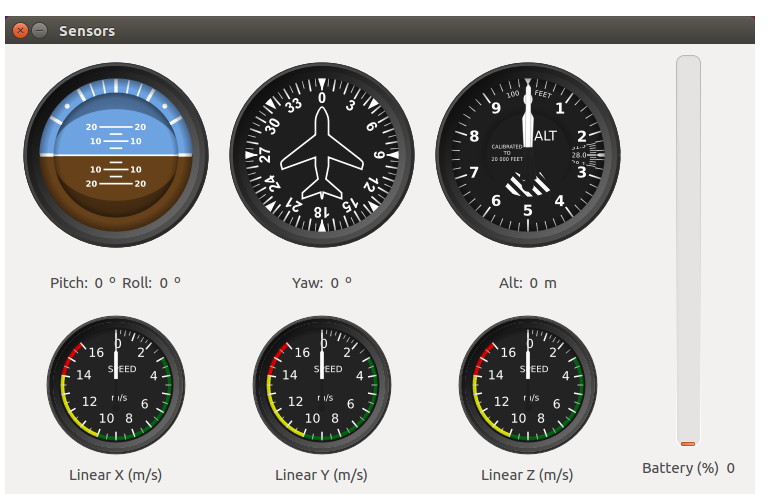
\includegraphics[scale=0.4]{imagenes/sensores.png}
  \caption{Interfaz gráfico de uav-viewer.py para mostrar los sensores}
  \label{fig:sensores}
\end{figure}

\section{Fichero de configuración}

La aplicación UAV-Viewer.py utiliza ficheros de configuración YAML. A continuación se muestra el fichero de configuración en el cuál se determinan en qué puertos específicos se comunica con los drivers, MAVLinkServer y cameraServer para intercambiar datos sensoriales y órdenes de control.

\begin{lstlisting}[frame=single]
Camera:
  Server: 1 # 0 -> Deactivate, 1 -> Ice , 2 -> ROS
  Proxy: "default -h 0.0.0.0 -p 9999"
  Format: RGB8
  Topic: "/MavLink/image_raw"
  Name: MavLinkCamera

Pose3D:
  Server: 1 # 0 -> Deactivate, 1 -> Ice , 2 -> ROS
  Proxy: "default -h 0.0.0.0 -p 9998"
  Topic: "/MavLink/Pose3D"
  Name: MavLinkPose3d

CMDVel:
  Server: 1 # 0 -> Deactivate, 1 -> Ice , 2 -> ROS
  Proxy: "default -h 0.0.0.0 -p 9997"
  Topic: "/MavLink/CMDVel"
  Name: MavLinkCMDVel

Navdata:
  Server: 1 # 0 -> Deactivate, 1 -> Ice , 2 -> ROS
  Proxy: "default -h 0.0.0.0 -p 9996"
  Topic: "/MavLink/Navdata"
  Name: MavLinkNavdata

Extra:
  Server: 1 # 0 -> Deactivate, 1 -> Ice , 2 -> ROS
  Proxy: "default -h 0.0.0.0 -p 9995"
  Topic: "/MavLink/Extra"
  Name: MavLinkExtra
\end{lstlisting}

\section{Experimentos}
Para cumplir con todos los requerimientos que pueden ser necesarios para la plataforma de JdeRobot, el visor que se ha desarrollado se ha validado con el 3DR Solo Drone.

Las primeras pruebas que se realizaron como se muestra en la figura \ref{fig:experimentoConUAV}\footnote{\url{https://www.youtube.com/watch?v=j5P7QywcFHk}} para validar el funcionamiento de la herramienta, fueron la realización de movimientos de traslación relativos, como puede ser avance o retroceso, ascenso o descenso, desplazamiento lateral en cualquier dirección y velocidades angulares (guiñada, alabeo, cabeceo).
\begin{figure}[H]
  \centering
  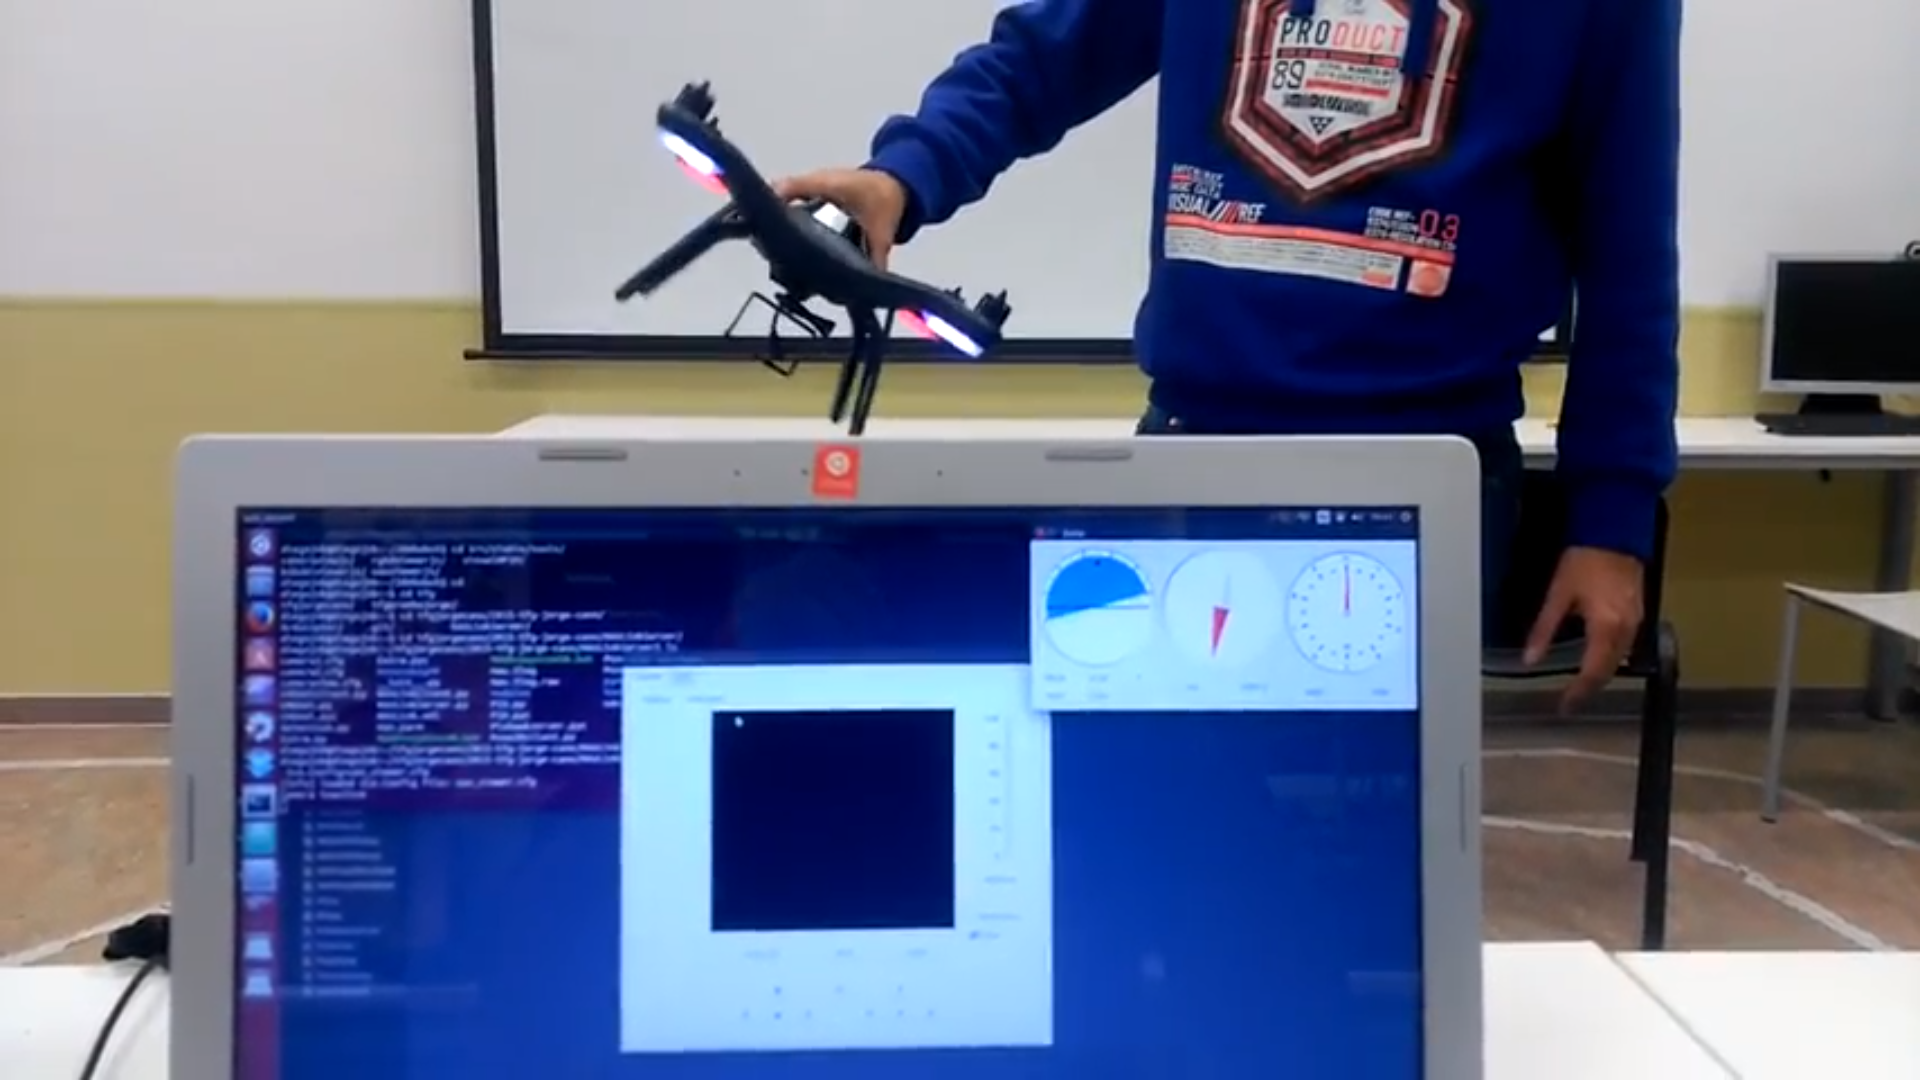
\includegraphics[scale=0.25]{imagenes/EXP1.png}
  \caption{Captación de movimientos del drone}
  \label{fig:experimentoConUAV}
\end{figure}
A continuación se implementó el sistema de aterrizaje y despegue. Para ello, se probó tanto en sitios abiertos como cerrados, pudiendo estudiar el efecto de las condiciones climáticas y las turbulencias generadas, sobre la actuación del dron.

Por último, se realizó una validación de los comandos de velocidad en dos pasos: el primero de ellos era comproborar que las órdenes que se enviaban, se recibían correctamente en el drone, para evitar accidentes; el segundo, como se ilustra en la figura \ref{fig:experimentoConjunto}\footnote{\url{https://www.youtube.com/watch?v=UtUWMH6s2Yk}}, consistía en probar el comportamiento de estos comandos en pleno vuelo para tomar medidas y a continuación realizar ajustes.   

\begin{figure}[H]
  \centering
  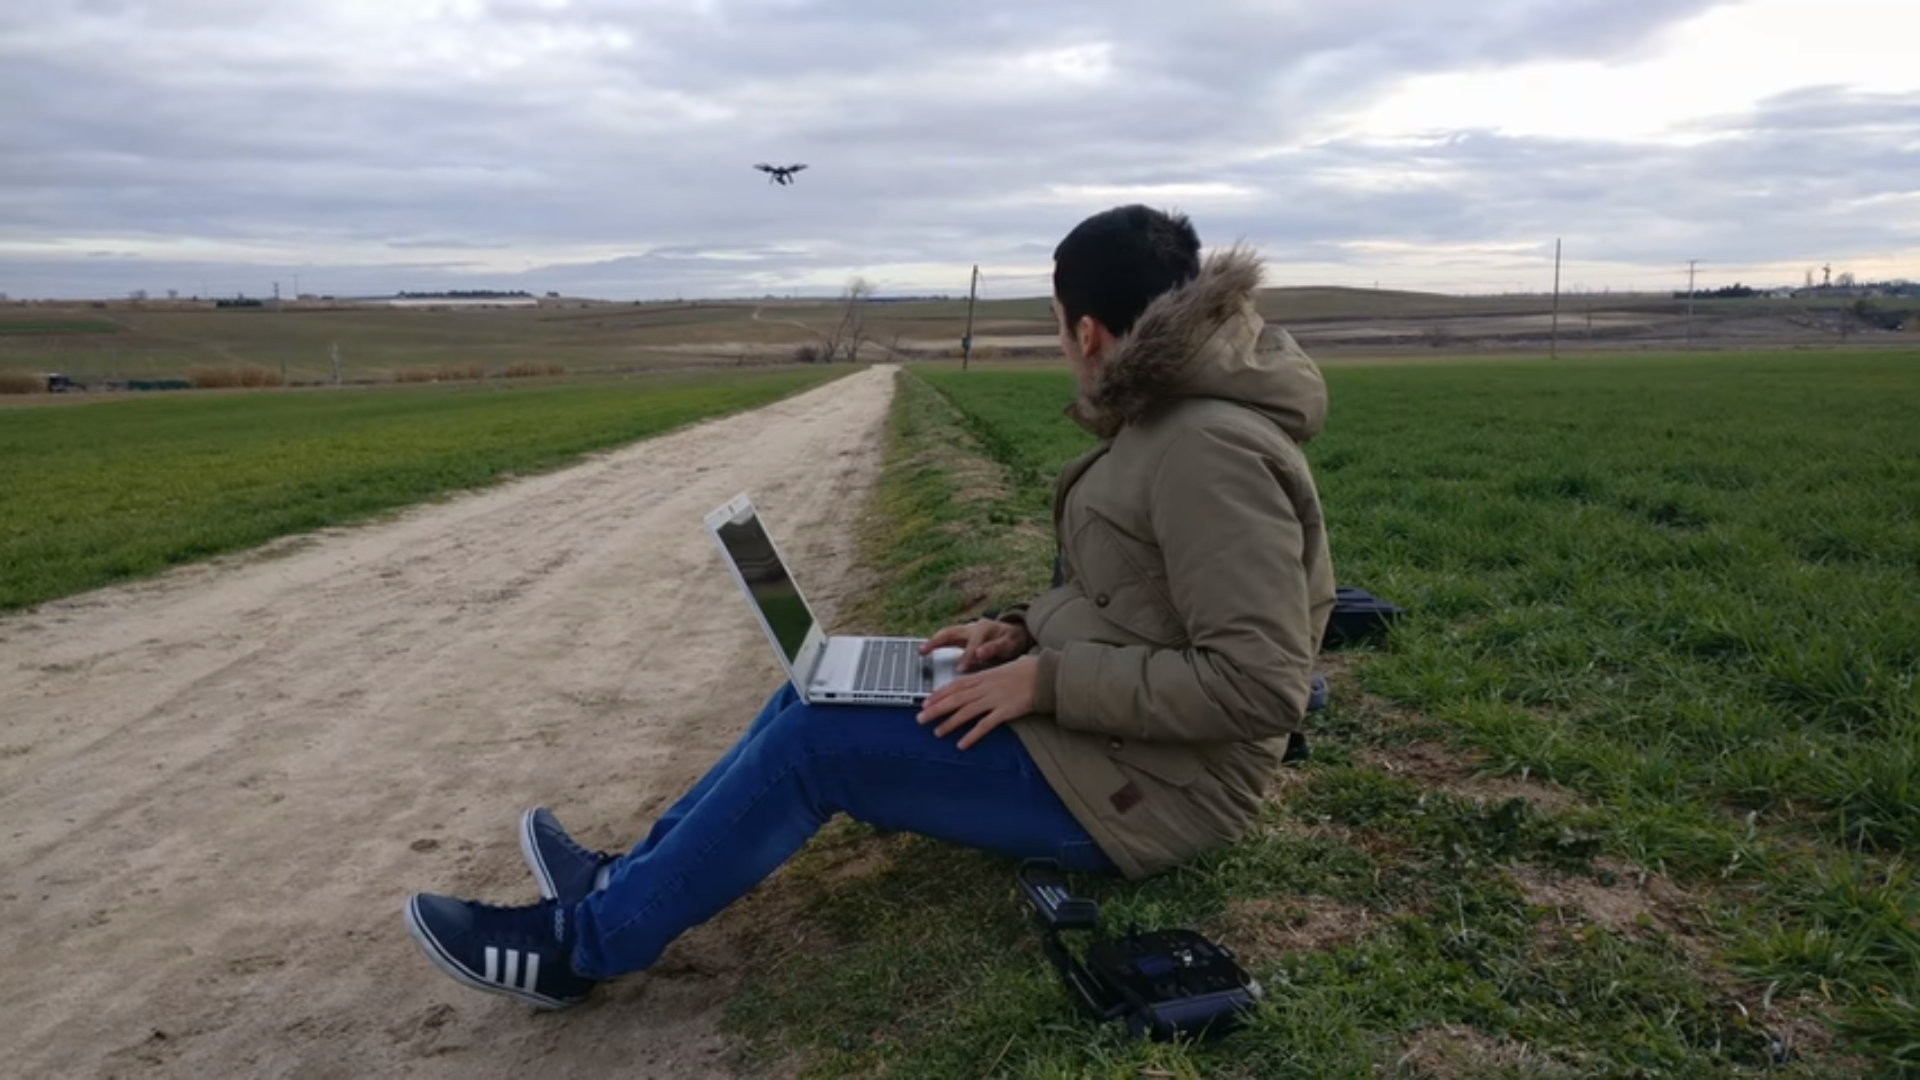
\includegraphics[scale=0.25]{imagenes/EXP2.png}
  \caption{Experimento de vuelo real}
  \label{fig:experimentoConjunto}
\end{figure}
